\documentclass[11pt, oneside]{article}   	% use "amsart" instead of "article" for AMSLaTeX format
\usepackage{geometry}                		% See geometry.pdf to learn the layout options. There are lots.
\geometry{letterpaper}                   		% ... or a4paper or a5paper or ... 
%\geometry{landscape}                		% Activate for rotated page geometry
%\usepackage[parfill]{parskip}    		% Activate to begin paragraphs with an empty line rather than an indent
\usepackage{graphicx}				% Use pdf, png, jpg, or eps§ with pdflatex; use eps in DVI mode
								% TeX will automatically convert eps --> pdf in pdflatex		
\usepackage{amssymb}
\usepackage{url}

%SetFonts

%SetFonts


\title{Homework 3}
\author{CS 4364/5364\\Spring 2021}
\date{Due: 11 March 2021}							% Activate to display a given date or no date

\begin{document}
\maketitle

Because of the reliance of the particular assignments in this class on mathematical notation, 
and the fact that all assignments will be submitted electronically, 
students are encouraged to use \LaTeX{} to formalize their responses. 
\textbf{For those enrolled in the graduate section the use of latex is \emph{required}.}
This assignment (like all others) will be posted on the course \texttt{github}\footnote{\url{github.com/deblasiolab/CS4364-documents}} as source code as well as in PDF form on the course website. 
Please submit your assignment to the professor via email, either as a link to your assignment online (i.e. overleaf or github) or as an attachment. 
Graduate students will need to include the \texttt{.tex} files as well as a PDF, this is optional but encouraged for undergraduates. 


\begin{enumerate}


\item \textbf{(30 points)} 
We know that just like the Suffix Tree and Suffix Array an BWT (and in turn an FM Index) can have contain the suffixes for more than one string. 
Assume we have constructed an FM Index for two strings. 
Assume that the first string is terminated by the character  \texttt{\#} and the second with \texttt{\$} (\texttt{\#} is lexicographically smaller than \texttt{\$}), neither of which is in $\Sigma$.
\begin{itemize}
\item Describe an algorithm to reconstruct all (both) strings contained in an FM Index. 
\item Use your algorithm to reconstruct the strings given the FM Index in Figure~\ref{fig:q1b} below. 
\item Describe an algorithm to use the same index to find out how many times a pattern $P$ is present in each of the strings (the output will be two different numbers). 
\end{itemize}

\begin{figure}
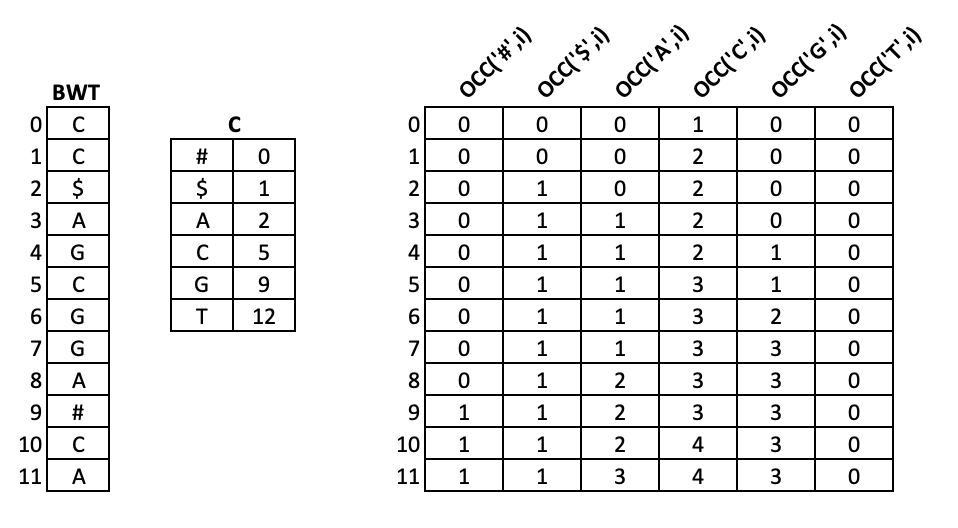
\includegraphics{HW3_FIG}
\caption{Example Ferragina Manzini Index}
\label{fig:q1b}
\end{figure}
\end{enumerate}
\end{document}  